\documentclass[a4paper,titlepage]{article}
\usepackage[utf8]{inputenc}
\usepackage{fullpage}
\usepackage{indentfirst}
\usepackage[per-mode=symbol]{siunitx}
\usepackage{listings}
\usepackage{graphicx}
\usepackage{color}
\usepackage{amsmath}
\usepackage{array}
\usepackage[hidelinks]{hyperref}
\usepackage[format=plain,font=it]{caption}
\usepackage{subcaption}
\usepackage{standalone}
\usepackage[nottoc]{tocbibind}
\usepackage{cleveref}
\usepackage{listings}
\usepackage{titlesec}
\usepackage{minted}
\usepackage{booktabs}
\usepackage{csvsimple}

% Custom commands
\newcommand\numberthis{\addtocounter{equation}{1}\tag{\theequation}}
\newcommand{\code}[1]{\texttt{#1}}
\newcolumntype{P}[1]{>{\centering\arraybackslash}p{#1}}

\setminted{linenos,breaklines,fontsize=\footnotesize}

%\titleformat*{\section}{\normalsize\bfseries}
%\titleformat*{\subsection}{\small\bfseries}
\renewcommand{\thesubsection}{\thesection.\alph{subsection}}
\providecommand*{\listingautorefname}{Listing}

%opening
\title{\textbf{ECSE 543 \\ Assignment 1}}
\author{Sean Stappas \\ 260639512}
\date{October 17, 2017}

\begin{document}
	\sloppy
	\maketitle
	\twocolumn
	
	\section{Introduction}
	
	The programs for this assignment were created in Python 2.7. The source code is provided as listings in \autoref{appendix:listings}. To perform the required tasks in this assignment, a custom matrix package was created, with useful methods such as add, multiply, transpose, etc. This package can be seen in \autoref{lst:matrices}. In addition, logs of the output of the programs are provided in \autoref{appendix:logs}.
	
	\section{Choleski Decomposition}
	
	\subsection{Choleski Program}
	% Write a program to solve the matrix equation Ax=b by Choleski decomposition. A is a real, symmetric, positive-definite matrix of order n.
	
	
	\subsection{Constructing Test Matrices}
	% Construct some small matrices (n = 2, 3, 4, or 5) to test the program. Remember that the matrices must be real, symmetric and positive-definite. Explain how you chose the matrices.
	
	\subsection{Test Runs}
	% Test the program you wrote in (a) with each small matrix you built in (b) in the following way: invent an x, multiply it by A to get b, then give A and b to your program and check that it returns x correctly.
	
	\subsection{Linear Networks}
	% Write a program that reads from a file a list of network branches (Jk, Rk, Ek) and a reduced incidence matrix, and finds the voltages at the nodes of the network. Use the code from part (a) to solve the matrix problem. Explain how the data is organized and read from the file. Test the program with a few small networks that you can check by hand. Compare the results for your test circuits with the analytical results you obtained by hand. Cleary specify each of the test circuits used with a labeled schematic diagram.
	% TODO: Put pictures of test circuits! (create your own as well as the provided ones…)
	
	\section{Finite Difference Mesh}
	
	\subsection{Equivalent Resistance}
	% Using the program you developed in question 1, find the resistance, R, between the node at the bottom left corner of the mesh and the node at the top right corner of the mesh, for N = 2, 3, …, 10. (You will probably want to write a small program that generates the input file needed by the network analysis program. Constructing by hand the incidence matrix for a 200-node network is rather tedious).
	
	\begin{table}[!htb]
		\centering
		\caption{Mesh equivalent resistance R versus mesh size N.}
		\csvautobooktabular{csv/q2a.csv}
		\label{tabel:q2a}
	\end{table}
	
	\subsection{Time Complexity}
	% In theory, how does the computer time taken to solve this problem increase with N, for large N? Are the timings you observe for your practical implementation consistent with this? Explain your observations.
	
	\begin{table}[!htb]
		\centering
		\caption{Runtime of mesh resistance solver program versus mesh size $N$.}
		\csvautobooktabular{csv/q2b.csv}
		\label{tabel:q2b}
	\end{table}

	\begin{figure}[!htb]
		\centering
		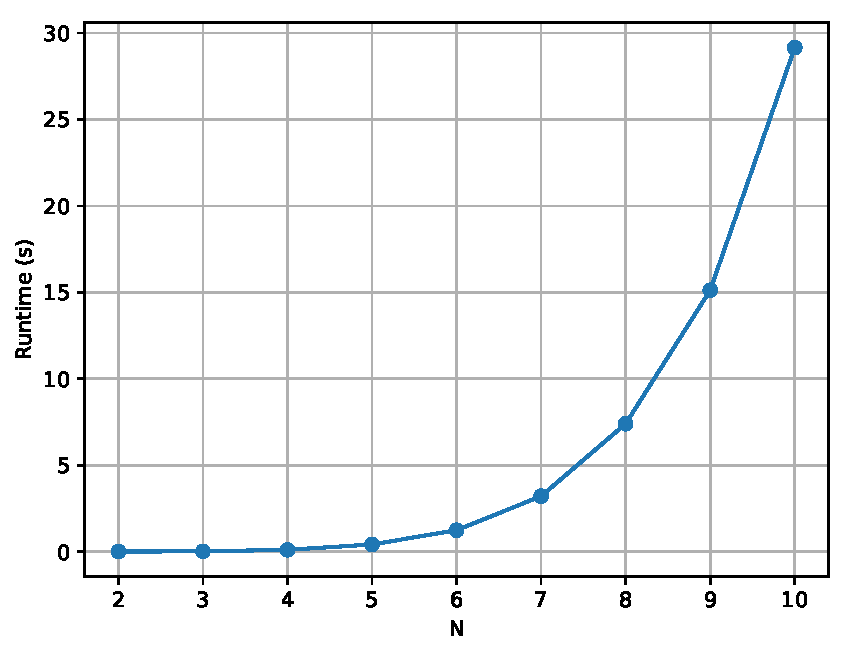
\includegraphics[width=\columnwidth]{plots/q2b.pdf}
		\caption
		{Runtime of mesh resistance solver program versus mesh size $N$.}
		\label{fig:q2b}
	\end{figure}
	
	\subsection{Sparsity Modification}
	% Modify your program to exploit the sparse nature of the matrices to save computation time. What is the half-bandwidth b of your matrices? In theory, how does the computer time taken to solve this problem increase now with N, for large N? Are the timings you for your practical sparse implementation consistent with this? Explain your observations.
	
	\begin{table}[!htb]
		\centering
		\caption{Runtime of banded mesh resistance solver program versus mesh size $N$.}
		\csvautobooktabular{csv/q2c.csv}
		\label{tabel:q2c}
	\end{table}

	\begin{figure}[!htb]
		\centering
		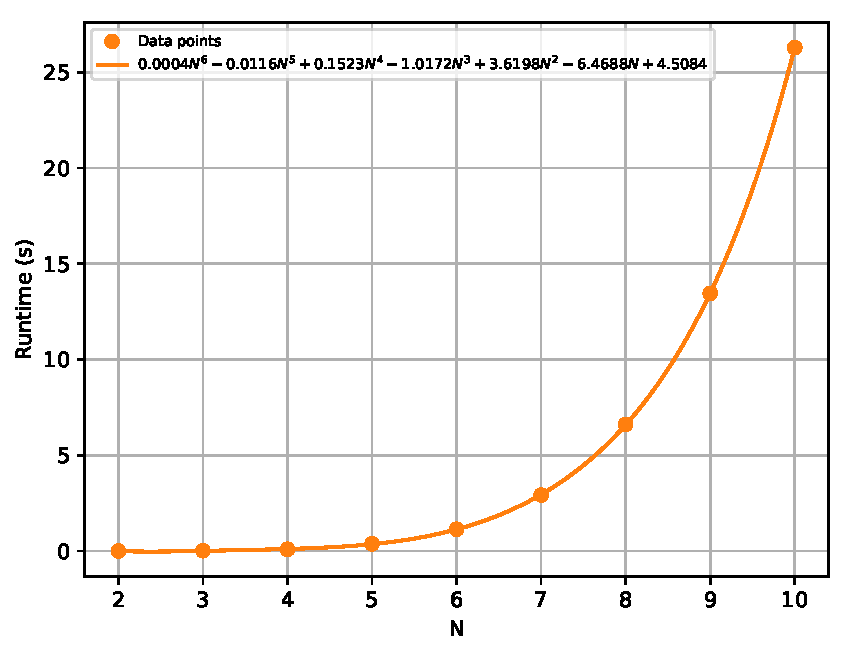
\includegraphics[width=\columnwidth]{plots/q2c.pdf}
		\caption
		{Runtime of banded mesh resistance solver program versus mesh size $N$.}
		\label{fig:q2c}
	\end{figure}

	\begin{figure}[!htb]
		\centering
		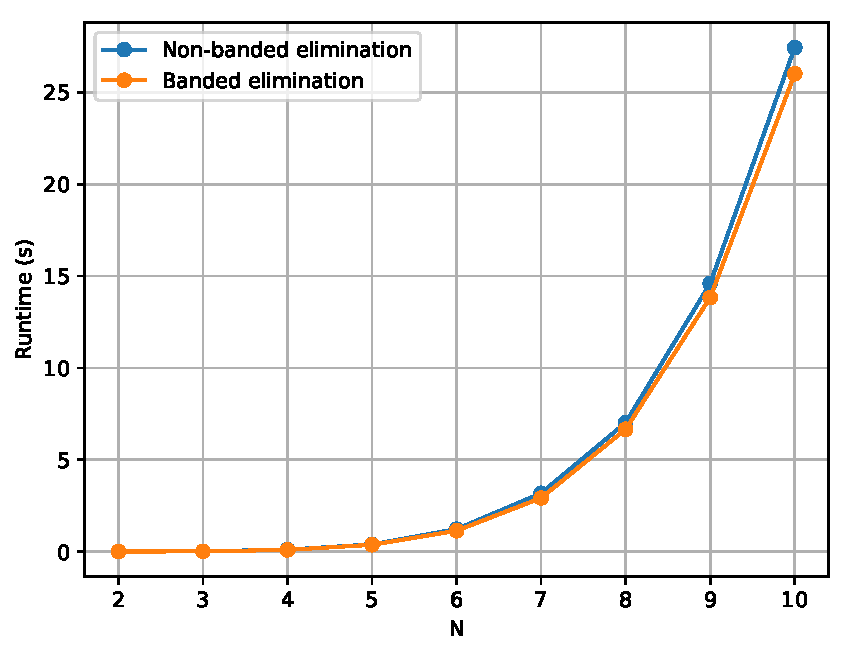
\includegraphics[width=\columnwidth]{plots/q2bc.pdf}
		\caption
		{Comparison of runtime of banded and non-banded resistance solver programs versus mesh size $N$.}
		\label{fig:q2bc}
	\end{figure}
	
	\subsection{Resistance vs. Mesh Size}
	% Plot a graph of R versus N. Find a function R(N) that fits the curve reasonably well and is asymptotically correct as N tends to infinity, as far as you can tell.
	
	% TODO: Fit log function to graph
	
	\begin{figure}[!htb]
		\centering
		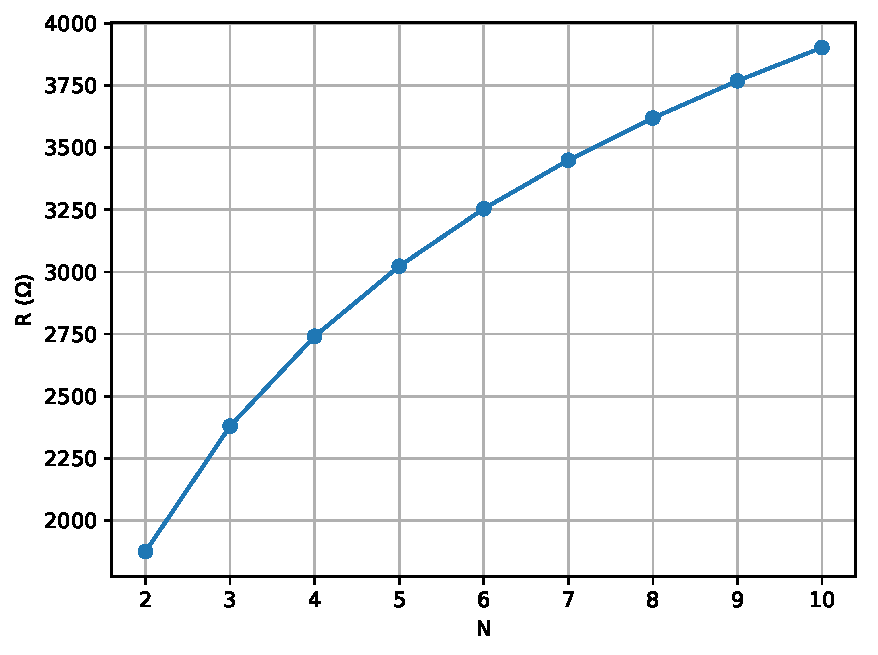
\includegraphics[width=\columnwidth]{plots/q2d.pdf}
		\caption
		{Resistance of mesh versus mesh size $N$.}
		\label{fig:q2d}
	\end{figure}
	
	\section{Coaxial Cable}
	
	\subsection{SOR Program}
	% Write a computer program to find the potential at the nodes of a regular mesh in the air between the conductors by the method of finite differences. Use a five-point difference formula. Exploit at least one of the planes of mirror symmetry that this problem has. Use an	equal node-spacing, h, in the x and y directions. Solve the matrix equation by successive	over-relaxation (SOR), with SOR parameter w. Terminate the iteration when the magnitude	of the residual at each free node is less than 10^-5.
	
	\subsection{Varying $\omega$}
	% With h = 0.02, explore the effect of varying w. For 10 values of w between 1.0 and 2.0,	tabulate the number of iterations taken to achieve convergence, and the corresponding value	of potential at the point (x ,y) = (0.06, 0.04). Plot a graph of number of iterations versus w.
	
	\begin{table}[!htb]
		\centering
		\caption{Number of iterations of SOR versus $\omega$.}
		\csvautobooktabular{csv/q3b_iterations.csv}
		\label{tabel:q3b_iterations}
	\end{table}
	
	\begin{figure}[!htb]
		\centering
		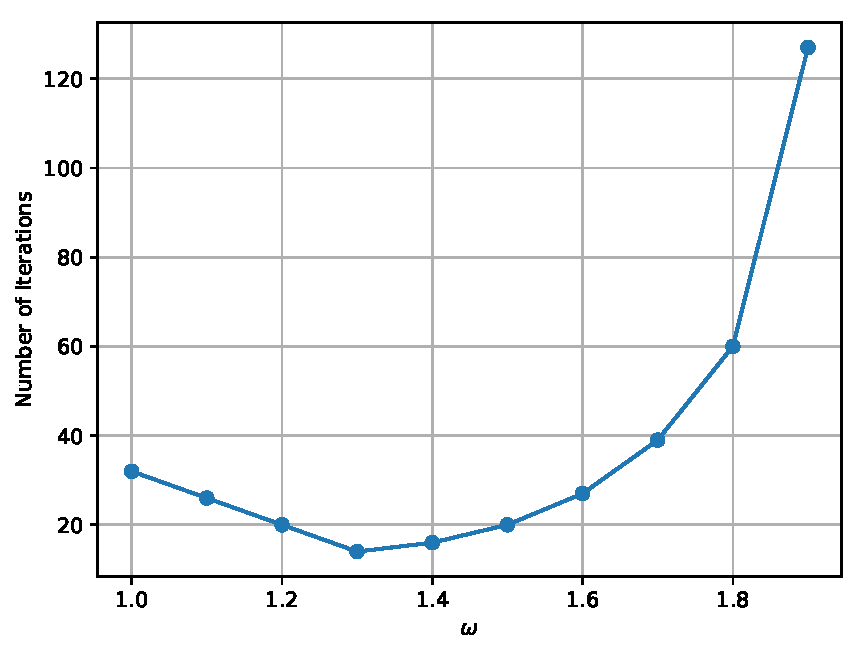
\includegraphics[width=\columnwidth]{plots/q3b.pdf}
		\caption
		{Number of iterations of SOR versus $\omega$.}
		\label{fig:q3b}
	\end{figure}

	\begin{table}[!htb]
		\centering
		\caption{Potential at (0.06, 0.04) versus $\omega$ when using SOR.}
		\csvautobooktabular{csv/q3b_potential.csv}
		\label{tabel:q3b_potential}
	\end{table}
	
	\subsection{Varying $h$}
	% With an appropriate value of w, chosen from the above experiment, explore the effect of	decreasing h on the potential. Use values of h = 0.02, 0.01, 0.005, etc, and both tabulate and	plot the corresponding values of potential at (x, y) = (0.06, 0.04) versus 1/h. What do you think is the potential at (0.06, 0.04), to three significant figures? Also, tabulate and plot the number of iterations versus 1/h. Comment on the properties of both plots.
	
	\begin{table}[!htb]
		\centering
		\caption{Number of iterations of SOR versus $1/h$. Note that $\omega=1.3$.}
		\csvautobooktabular{csv/q3c_iterations.csv}
		\label{tabel:q3c_iterations}
	\end{table}
	
	\begin{figure}[!htb]
		\centering
		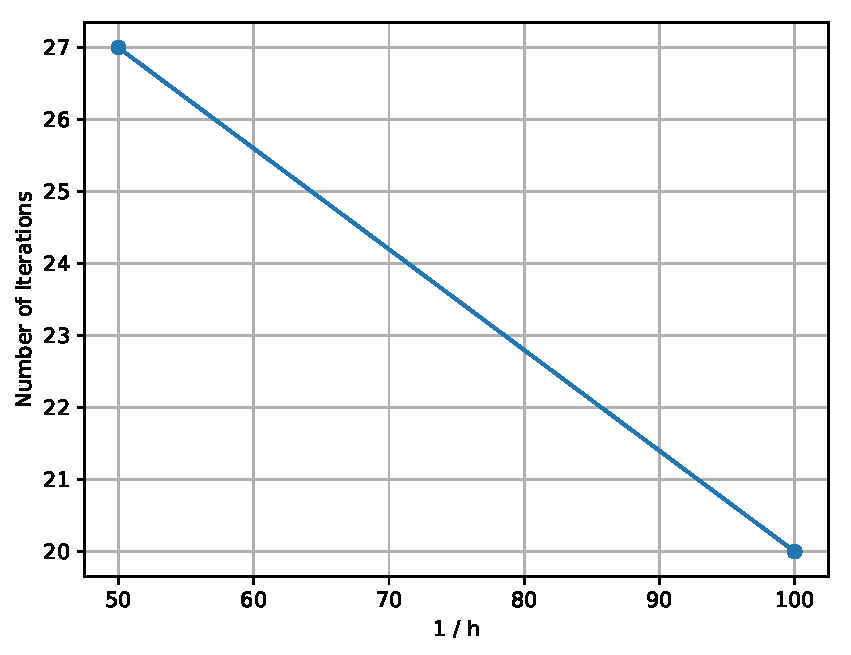
\includegraphics[width=\columnwidth]{plots/q3c_iterations.pdf}
		\caption
		{Number of iterations of SOR versus $1/h$. Note that $\omega=1.3$.}
		\label{fig:q3c_iterations}
	\end{figure}

	\begin{table}[!htb]
		\centering
		\caption{Potential at (0.06, 0.04) versus $1/h$ when using SOR.}
		\csvautobooktabular{csv/q3c_potential.csv}
		\label{tabel:q3c_potential}
	\end{table}

	\begin{figure}[!htb]
		\centering
		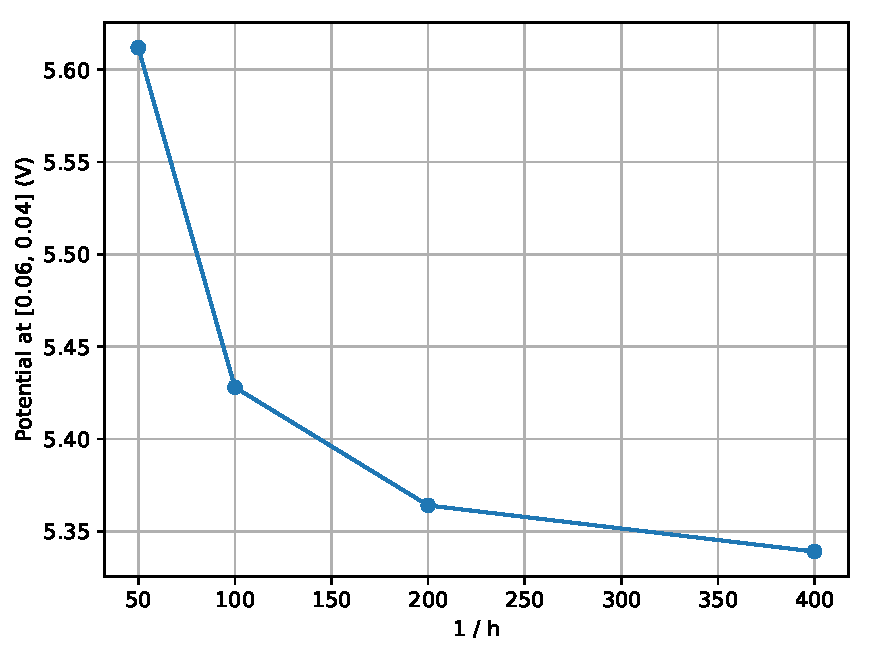
\includegraphics[width=\columnwidth]{plots/q3c_potential.pdf}
		\caption
		{Potential at (0.06, 0.04) found by SOR versus $1/h$. Note that $\omega=1.3$.}
		\label{fig:q3c_potential}
	\end{figure}
	
	\subsection{Jacobi Method}
	% Use the Jacobi method to solve this problem for the same values of h used in part (c). Tabulate and plot the values of the potential at (x, y) = (0.06, 0.04) versus 1/h and the number of iterations versus 1/h. Comment on the properties of both plots and compare to those of SOR.
	
	\begin{table}[!htb]
		\centering
		\caption{Number of iterations versus $\omega$ when using the Jacobi method.}
		\csvautobooktabular{csv/q3d_iterations.csv}
		\label{tabel:q3d_iterations}
	\end{table}

	\begin{figure}[!htb]
		\centering
		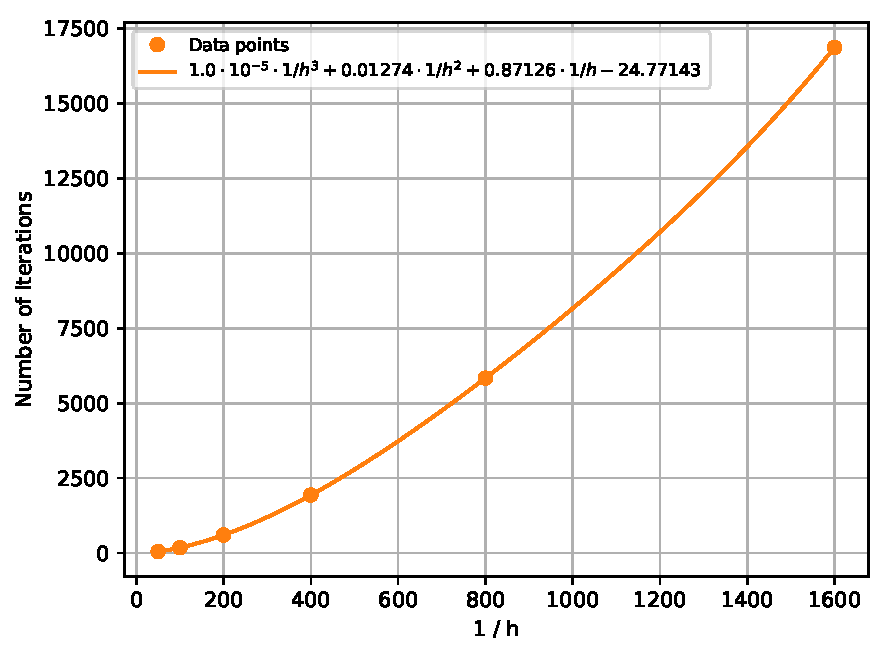
\includegraphics[width=\columnwidth]{plots/q3d_iterations.pdf}
		\caption
		{Number of iterations of the Jacobi method versus $1/h$.}
		\label{fig:q3d_iterations}
	\end{figure}

	\begin{table}[!htb]
		\centering
		\caption{Potential at (0.06, 0.04) versus $1/h$ when using the Jacobi method.}
		\csvautobooktabular{csv/q3d_potential.csv}
		\label{tabel:q3d_potential}
	\end{table}

	\begin{figure}[!htb]
		\centering
		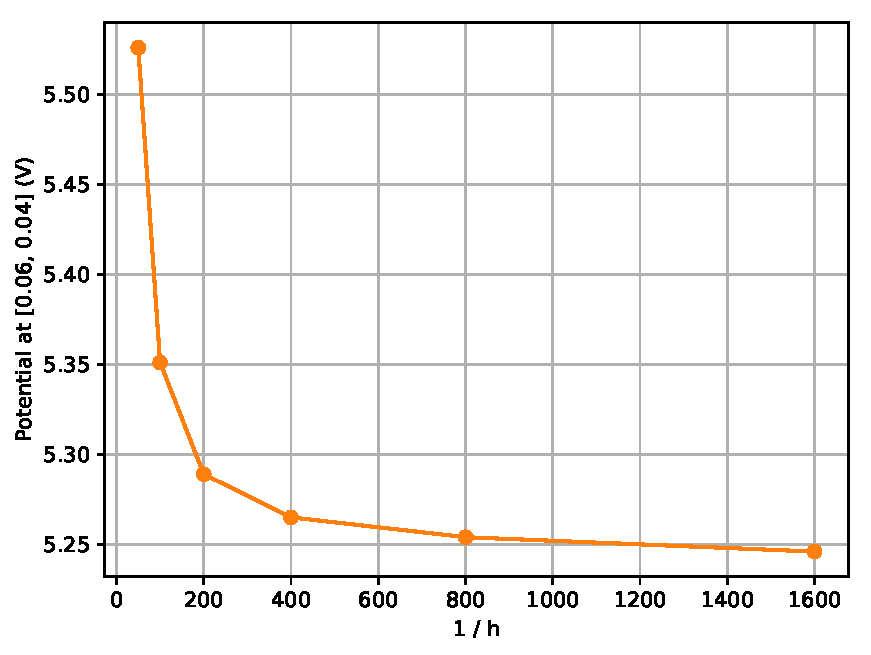
\includegraphics[width=\columnwidth]{plots/q3d_potential.pdf}
		\caption
		{Potential at (0.06, 0.04) versus $1/h$ when using the Jacobi method.}
		\label{fig:q3d_potential}
	\end{figure}

	\begin{figure}[!htb]
		\centering
		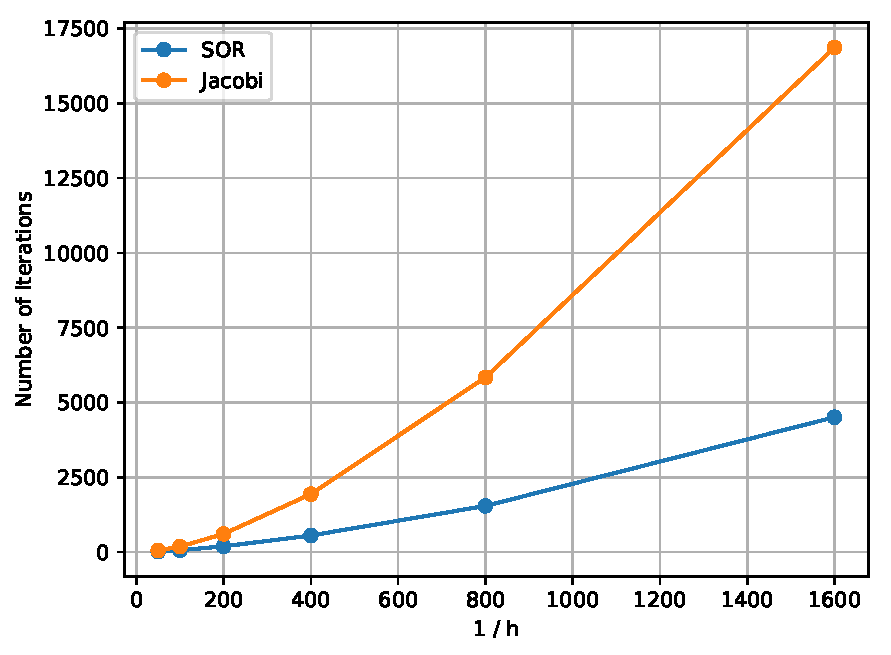
\includegraphics[width=\columnwidth]{plots/q3d_iterations_comparison.pdf}
		\caption
		{Comparison of number of iterations when using SOR and Jacobi methods versus $1/h$. Note that $\omega=1.3$ for the SOR program.}
		\label{fig:q3d_iterations_comparison}
	\end{figure}
	
	\subsection{Non-uniform Node Spacing}
	% Modify the program you wrote in part (a) to use the five-point difference formula derived in	class for non-uniform node spacing. An alternative to using equal node spacing, h, is to use	smaller node spacing in more “difficult” parts of the problem domain. Experiment with a	scheme of this kind and see how accurately you can compute the value of the potential at (x, y)	= (0.06, 0.04) using only as many nodes as for the uniform case h = 0.01 in part (c).

	\onecolumn
	
	\appendix
	
	\section{Code Listings} \label{appendix:listings}
	
	\begin{center}
		\captionof{listing}{Custom matrix package.}
		\inputminted{python}{../matrices.py}
		\label{lst:matrices}
	\end{center}

	\begin{center}
		\captionof{listing}{Linear resistive networks.}
		\inputminted{python}{../linear_networks.py}
		\label{lst:linear_networks}
	\end{center}
	
	\begin{center}
		\captionof{listing}{Finite difference method.}
		\inputminted{python}{../finite_diff.py}
		\label{lst:finite_diff}
	\end{center}
	
	\begin{center}
		\captionof{listing}{Question 1.}
		\inputminted{python}{../q1.py}
		\label{lst:q1}
	\end{center}
	
	\begin{center}
		\captionof{listing}{Question 2.}
		\inputminted{python}{../q2.py}
		\label{lst:q2}
	\end{center}

	\begin{center}
		\captionof{listing}{Question 3.}
		\inputminted{python}{../q3.py}
		\label{lst:q3}
	\end{center}

	\section{Output Logs} \label{appendix:logs}
	
	\begin{center}
		\captionof{listing}{Output of Question 1 program.}
		\inputminted{pycon}{logs/q1.txt}
		\label{lst:q1_log}
	\end{center}

	\begin{center}
		\captionof{listing}{Output of Question 2 program.}
		\inputminted{pycon}{logs/q2.txt}
		\label{lst:q2_log}
	\end{center}
	
	\begin{center}
		\captionof{listing}{Output of Question 3 program.}
		\inputminted{pycon}{logs/q3.txt}
		\label{lst:q3_log}
	\end{center}

\end{document}
